%\section{Выбор  языка программирования}
%Выбранный язык – С++.
%Причины:
%\begin{enumerate}
%	 \item Компилируемый язык со статической типизацией. 
%	 \item Сочетание высокоуровневых и низкоуровневых средств.
%	 \item Реализация ООП.
%	 \item Наличие удобной стандартной библиотеки шаблоны
%	 \end{enumerate}
%\section{Выбор вспомогательных библиотек}
%Для реализации программы была выбрана библиотека Qt.
%\begin{enumerate}
%	\item Широкие возможности работы с изображениями, в том числе и попиксельно
%	\item Наличии более функциональных аналогов стандартной библиотеки шаблонов в том числе для разнообразных структур данных
%\end{enumerate}
%\subsection{Диаграмма классов}
%\begin{figure}[h!]
%	\centering
%	\includegraphics[width=\textwidth]{img/diagramm.png}
%	\caption{Диаграмма классов}
%	\label{fig:spire03}
%\end{figure}

%%% Local Variables:
%%% mode: latex
%%% TeX-master: "rpz"
%%% End:

\chapter{Технологический раздел}

В данном разделе будут рассмотрены детали реализации программного комплекса, описанного в конструкторской части работы, и приведены примеры 
работы программы.

\section{Выбор и обоснование средств разработки}
В качестве языка программирования, на котором будет реализовано программное обеспечение, выбран язык C++ \cite{cpp}.
Данный выбор обусловлен следующими причинами:
\begin{enumerate}
	\item[1)] высокая скорость работы языка;
	\item[2)] строгая типизация;
	\item[3)] наличие библиотек для работы с микроконтроллерами семейства STM32 и периферийными устройствами;
	\item[4)] наличие большого количества материалов о разработке программного обеспечения для микроконтроллеров семейства STM32 на данном языке;
	\item[5)] возможность сертификации программ, написанных на данном языке \cite{fstec}.
\end{enumerate}

В качестве среды разработки был выбран текстовый редактор Visual Studio Code \cite{vscode}, обладающий большим количеством плагинов 
и инструментов для создания программного обеспечения на различных языках, в том числе на C++.

Для контроля качества кода использовался статический анализатор кода cppcheck \cite{cppcheck} и отладчик использования памяти 
valgrind \cite{valgrind}.



\section{Формат задания исходных данных}
Разработанный графический инструмент использует полигональное представление трёхмерных моделей. Для их задания необходима информация 
о полигонах, из которых состоит модель, а именно их геометрическое строение и цвет. Также для построения трёхмерной сцены необходима 
информация о расположении источников света.

\subsection{Задание геометрии трёхмерных моделей}
В качестве формата, задающего геометрическое строение и расположение полигонов на сцене, был выбран формат obj \cite{obj}. Это  простой 
формат данных, который представляет только трехмерную геометрию, а именно координаты вершин, индексы вершин, 
составляющие полигоны, а также текстуры и нормали. Важно заметить, что с форматом obj могут работать различные редакторы 
трёхмерной графики. Самыми популярными среди них являются Blender \cite{blender}, Autodesk AutoCAD \cite{autocad}, 
Adobe Photoshop \cite{photoshop} и КОМПАС-3D \cite{compass}. Пример файла формата obj приведён в приложении \ref{cha:appendix3} 
(листинг \ref{lst:cube_obj}).

\subsection{Задание характеристик материалов}
Формат obj помимо геометрии задаёт материалы, из которых выполнены заданные полигоны. Эти материалы подробно описывает формат 
mtl \cite{mtl}, который содержит в себе информацию о цвете и оптических свойствах полигонов, из которых состоит трёхмерная модель. 
Пример файла формата mtl приведён в приложении \ref{cha:appendix3} (листинг \ref{lst:cube_mtl}).

\subsection{Задание источников света}
Форматы obj и mtl описывают только трёхмерные модели не предусматривают задания расположения источников света на сцене. Поэтому 
для представления этих данных был разработан формат lgt, в котором построчно задаются вещественные координаты x, y, z источников света. 
Пример файла формата lgt приведён в приложении \ref{cha:appendix3} (листинг \ref{lst:cube_lgt}).



\section{Структура программы}
В программе реализованы следующие модули:
\begin{description}
	\item[reader] модуль чтения исходных данных из файлов;
	\item[converter] модуль подготовки исходных данных для алгоритмов визуализации;
	\item[writer] модуль записи сконвертированных данных в промежуточный файл;
	\item[display] модуль, предоставляющий данные о конкретном дисплее и функции для работы с ним;
	\item[errors] модуль обработки ошибок;
	\item[debug] отладочный модуль;
	\item[warnock] модуль, реализующий алгоритм Варнока удаления невидимых линий и поверхностей;
	\item[wstack] модуль, предоставляющий структуры данных "окно"{}, "стек окон"{} и операции над ними;
	\item[data\_structures] модуль, предоставляющий структуры данных, описывающие полигональные модели.
\end{description}

Диаграмма модулей программы представлена на рисунке \ref{fig:modules}.

\begin{figure}[h]
	\centering
	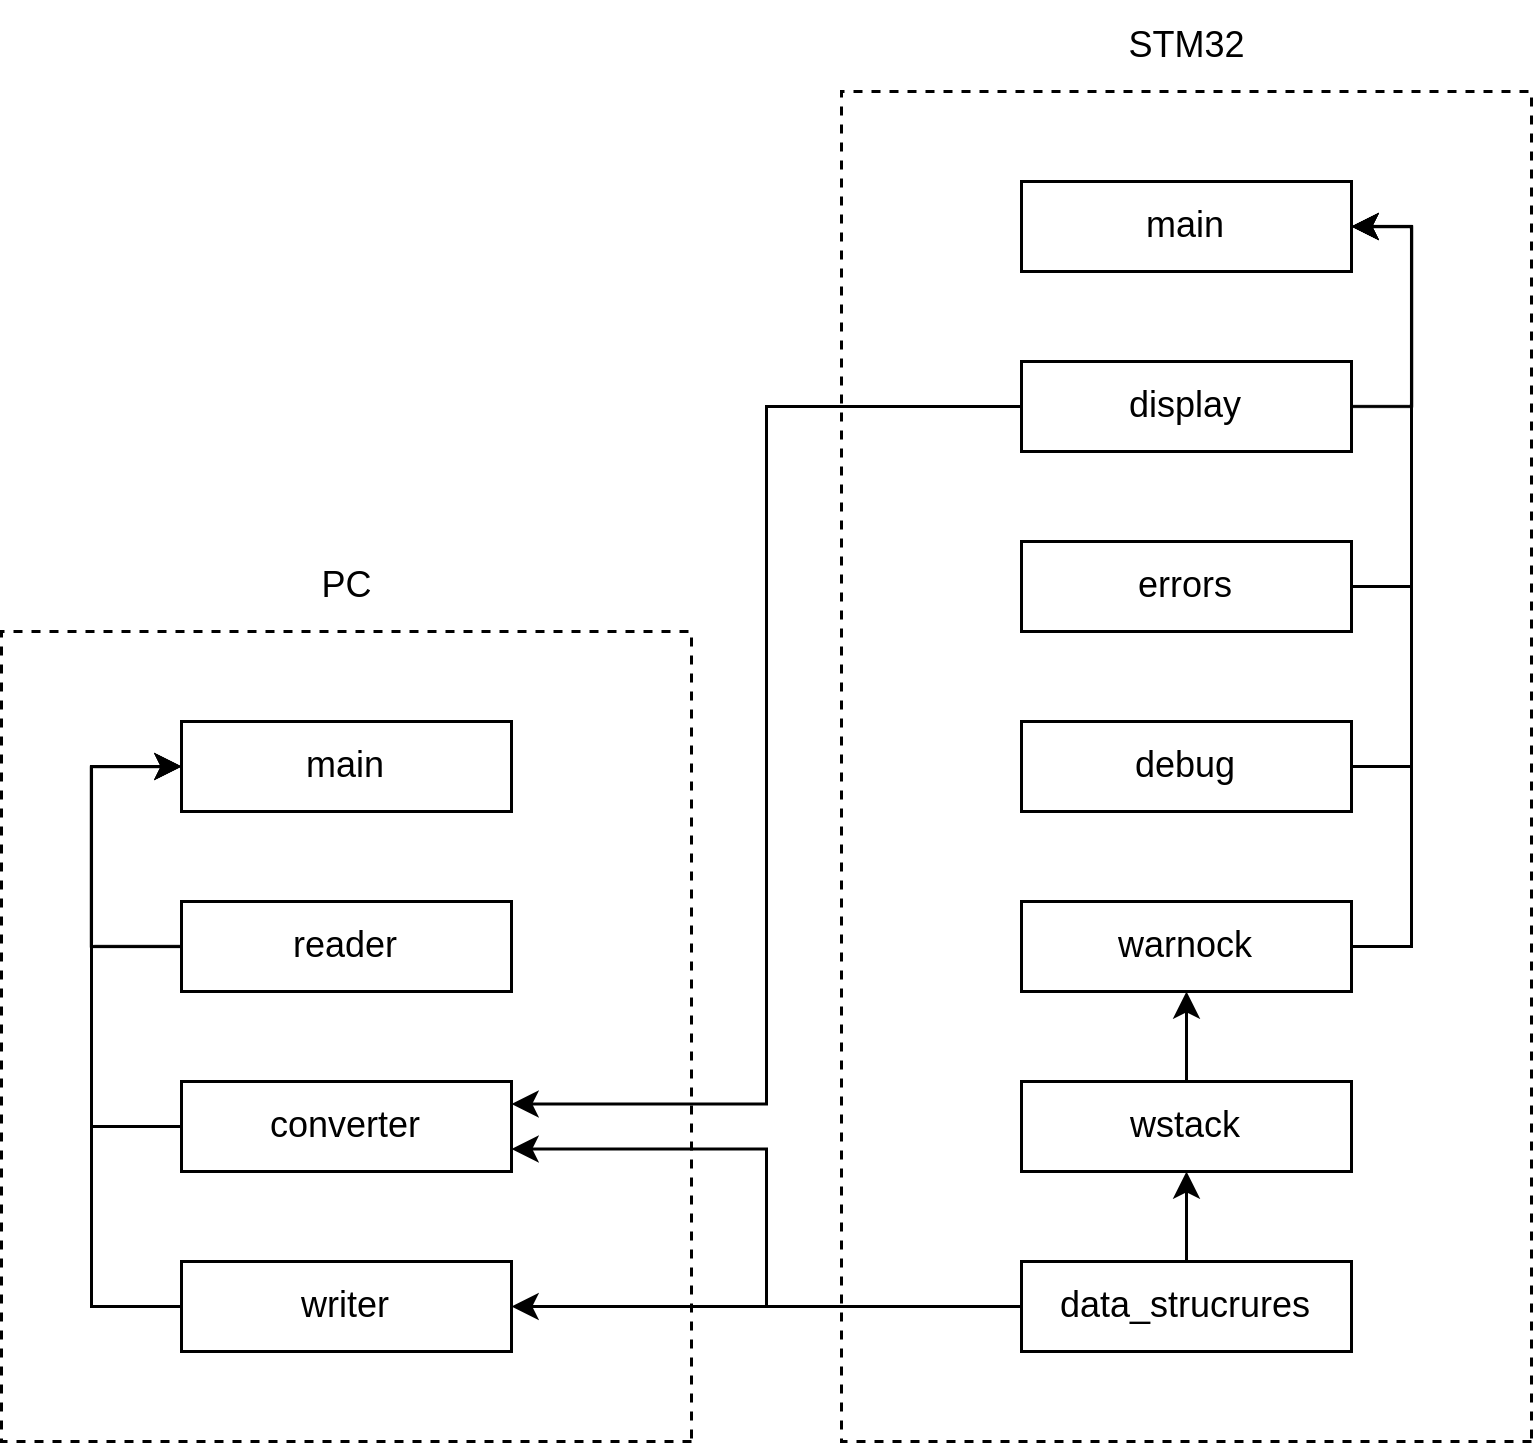
\includegraphics[width=\textwidth ]{img/modules/modules.png}
	\caption{Диаграмма модулей программы}
	\label{fig:modules}
\end{figure} 

Программа разделена на две части. Первая предназначена для предобработки исходных данных и выполняется на компьютере. Она получает на вход 
файлы с исходными данными и транслирует их в файл, который компонуется со второй частью программы, отвечающей за рендеринг изображения. 
Получившаяся программа загружается на микроконтроллер и выводит на дисплей заданное изображение.

Такая гибкая архитектура позволяет заменять аппаратное обеспечение, на котором должна выполняться программа, не затрагивая при этом 
алгоритмы рендеринга трёхмерной сцены. Это означает, что данное программное обеспечение обладает достаточно большой универсальностью
с точки зрения требований к аппаратному обеспечению и не зависит от конкретных моделей микроконтроллера и дисплея.

Также для развёртывания и запуска программы был написан сценарий сборки, предназначенный для запуска на операционных системах 
семейства Linux \cite{linux}.



\section{Детали реализации алгоритмов}
В листинге \ref{lst:warnock} представлен код функции warnock\_subdivide, которая реализует алгоритм Варнока удаления 
невидимых линий и поверхностей.
% \newpage
\lstinputlisting[language=C,caption=Алгоритм Варнока,label=lst:warnock]{listings/warnock.cpp}

Перед анализом каждого окна выполняется идентификация многоугольников с целью их разделения на три группы: внешние, 
охватывающие и все остальные. В том случае, если необходимо разбиение окна, оно делится на четыре равные части, если это возможно. 
Перед разбиением из массива многоугольников удаляются внешние, так как они заведомо будут внешними относительно подокон и 
не будут играть никакой роли при изображении сцены. Данная оптимизация повышает быстродействие алгоритма.

\section{Взаимодействие с программой}
Для программы был разработан консольный интерфейс, а не графический. Такое решение было принято по причине выбора формата задания 
исходных данных, не требующего от пользователя большого количества действий. Также консольный интерфейс позволяет использовать 
разработанный программный инструмент другими программами. В будущем это позволит разрабатывать программное обеспечение для семейства 
микроконтроллеров STM32, использующее трёхмерную графику.

Для запуска программы необходимо выполнить четыре шага: установить зависимости, подготовить исходные данные, подключить 
микроконтроллер к компьютеру и запустить рендеринг.

\subsection{Установка зависимостей}
Ввиду того, что для изменения выводимого на дисплей изображения программу приходится перекомпоновывать, на компьютере, с которого 
будет загружаться программа, должны быть установлены инструменты, необходимые для компоновки программы \cite{toolchain}. 
Также для запуска сценария сборки требуется утилита make \cite{make}.

\subsection{Подготовка исходных данных}
Рассмотрим данный и последующие этапы на примере модели куба. Для задания трёхмерных моделей необходимо создать 3 файла. 
Содержимое файлов cube.obj, cube.mtl и cube.lgt приведено в приложении \ref{cha:appendix3}. Первые два файла можно экспортировать 
из графических редакторов, а третий создать с помощью текстового редактора. Полученные файлы необходимо поместить в директорию 
проекта models/название\_модели (в примере директория будет называться models/cube).

\subsection{Подключение микроконтроллера}
Для загрузки программы на микроконтроллер необходимо подключить его к компьютеру с помощью проводного соединения и запомнить 
абсолютный путь к файлу устройства.

\subsection{Запуск программы}
Для запуска сборки необходимо выполнить в командной оболочке команду вида 
\lstinputlisting[language=bash,numbers=none]{listings/deploy.sh}
% \text{sudo make view model=cube device=/dev/sdb target=/run/media/inspirate/NODE\_F767ZI,}
где model - название модели, device - файл подключенного устройства, target - точка монтирования устройства. 
Далее произойдёт компиляция программы, после чего она загрузится на микроконтроллер и выведет изображение на дисплей. 



\section{Примеры работы программы}
На рисунке \ref{fig:cube} приведено изображение модели куба, рассматриваемое в качестве примера. Другие изображения моделей приведены в 
приложении \ref{cha:appendix4}.

\newpage
\begin{figure}[h]
	\centering
	\includegraphics[width=\textwidth ]{img/models/cube_with_hardware.jpg}
	\caption{Изображение модели куба на дисплее с разрешением 320x240 пикселей}
	\label{fig:cube}
\end{figure} 





\section{Вывод из технологического раздела}
В данном разделе были рассмотрены детали реализации программного инструмента, разработанного на основе алгоритма Варнока удаления 
невидимых линий и поверхностей. Также был рассмотрен алгоритм взаимодействия с программой и были приведены примеры её работы.
